\section{Pattern Language}

This section describes subset of PltRedex's pattern specification language supported by \texttt{PyPltRedex}. Grammar for the pattern language can be seen in Figure \ref{pattern-grammar}, in EBNF notation. 

\begin{figure}[h]
\begin{minted}[tabsize=2,obeytabs,escapeinside=//,mathescape=true,fontsize=\normalsize]{text}
pattern = number 
        | integer 
        | real 
        | natural 
        | string 
        | boolean 
        | variable-not-otherwise-mentioned 
        | hole 
        | symbol
        | (in-hole pattern pattern)
        | (pattern-sequence *) 

pattern-sequence : pattern 
                 | pattern ...  # literal ellipsis
\end{minted}
\caption{Grammar of the pattern language.}
\label{pattern-grammar}
\end{figure}

\begin{itemize}
\item
\textit{number} pattern matches any number.

\item
\textit{integer} matches any exact integer. 

\item
\textit{real} matches any real number.

\item
\textit{natural} matches any natural number; that is, any non-negative integer.

\item
\textit{string} matches any string.

\item
\textit{boolean} matches any boolean \texttt{\#t} or \texttt{\#f}.
\item
\textit{variable-not-otherwise-mentioned} matches any symbol that is not used as a literal in the language definition. For example, if language definition contains the pattern \texttt{(+ number number)} \textit{variable-not-otherwise-mentioned} will not match symbol \texttt{+}.

\item
\textit{hole} matches \texttt{hole} term exactly.

\item
\textit{symbol} matches any symbol except if its value coincides with non-terminal symbol in the language definition or contains an underscore.
\end{itemize}

All patterns above, except \textit{hole} can be suffixed with underscore and identifier (for example, \textit{number\_1}) to create binding to matched term.

\begin{itemize}
\item
\textit{(in-hole pattern pattern)} traverses the term trying to match the second pattern; upon successful match the term matching the second pattern is replaced with the term \texttt{hole} and then the first pattern is matched. The first pattern must match exactly one hole.

\item
\textit{pattern-sequence} pattern matches a term list, where each pattern-sequence element matches an element of the list. Each individual pattern within the sequence can be suffixed with \texttt{...} (literal ellipsis) and that will match zero or more terms matching the pattern.

Ellipses may produce non-deterministic matches. For example, consider a pattern \texttt{(number\_1 ... number\_2)} and a term \texttt{(1 2)}. There are three resulting matches: \texttt{(number\_1 : (), number\_2: (1 2))}, \texttt{(number\_1 : (1), number\_2: (2))}, and \texttt{(number\_1 : (1 2), number\_2: ())}. In the first case, \texttt{number\_1 ...} matches zero terms that match the pattern \texttt{number\_1} and hence pattern \texttt{number\_2} has to match remaining numbers. In the second case, \texttt{number\_1} matches a term \texttt{1}, and hence the term \texttt{2} is matches by \texttt{number\_2 ...}. Lastly, \texttt{number\_1} may match all the numbers in the sequence, leaving nothing for pattern \texttt{number\_2 ...} to consume.
\end{itemize}

If patterns in the pattern-sequence are suffixed with the same identifier (e.g. \texttt{(number\_1 number\_1)})), then the match is constrained to terms that are equal. That means term \texttt{(1 1)} matches the pattern but \texttt{(1 2)} does not. For patterns in a \texttt{define-language} form constraint checking is not performed. PLTRedex provides other constraint checks but they will not be considered.

\section{Compile-Time Representation of Patterns}

Throughout the report the following notation will be used to represent the Python classes used in the implementation of the pattern language. It follows the following format: \mintinline{text}{Typename(|$a$|: A, [|$b_1,...,b_n$|]: B, [|$c_1,...,c_m$|]: C?)}. $a$ is a field of type \texttt{A}. \mintinline{text}{[|$b_1,...,b_n$|]} is a sequence containing $n$ fields of type \texttt{B}. \mintinline{text}{[|$c_1,...,c_m$|]} is a sequence containing \textit{zero} or $m$ fields of type \texttt{C} (that is, \texttt{C?} is an optional type).

\begin{figure}[H]
	\centering
	\makebox[\textwidth][c] { 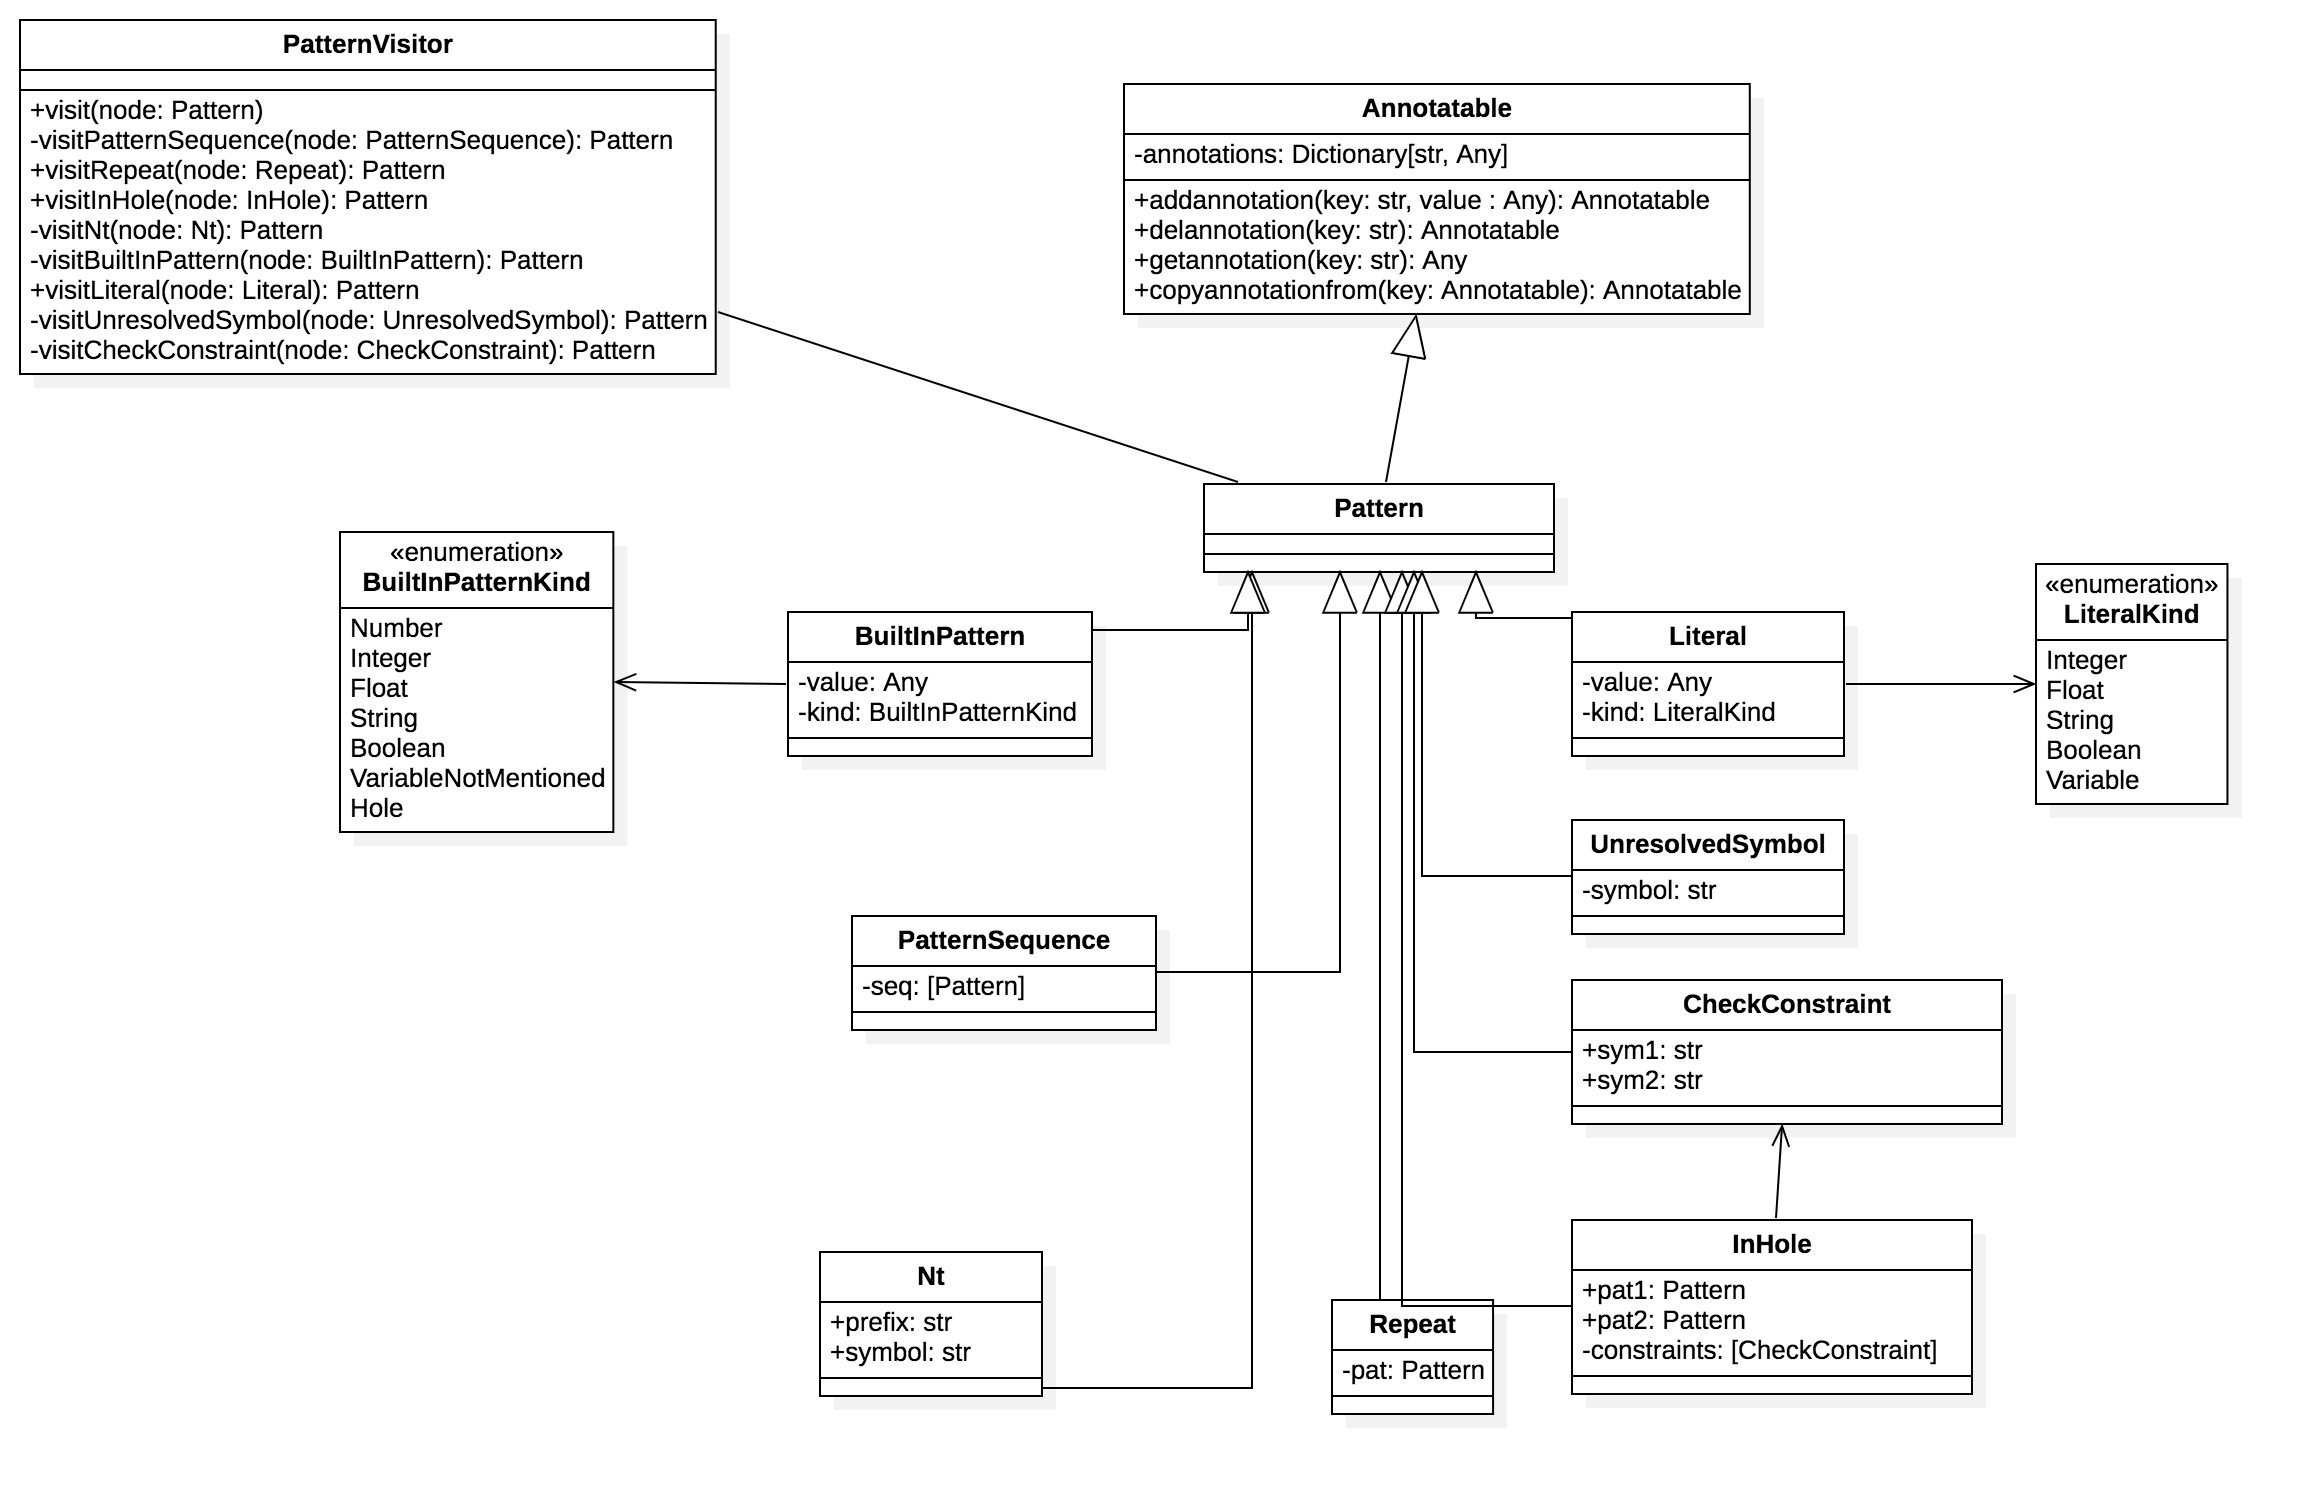
\includegraphics[scale=0.23]{class-diagram-pattern.png} }
	\caption{Representation of patterns.}
\label{class-diagram-pattern}
\end{figure}

Figure \ref{class-diagram-pattern} shows class diagram for all patterns.

\begin{itemize}
\item
\PatternSequence \space represents the \texttt{pattern-sequence} clause of the pattern language and may contain zero or more child patterns $p_i$. 

\item 
\PatternRepeat \space represents pattern $p_r$ under ellipsis.

\item
\PatternCheckConstraint is used for equality checking of terms. Terms assigned to $sym_1$ and $sym_2$ are checked for equality.

\item 
\NonTerminal \space represents non-terminal. $nt$ is a non-terminal symbol, while $pv$ is a pattern-variable to which some term will be assigned during matching. 

\item
\BuiltInPattern \space represents various built-in patterns such as \texttt{number} or \texttt{string}. $tag$ is chosen from \texttt{BuiltInPatternKind} enumeration.

\item
\PatternInHole \space represents \texttt{in-hole} pattern where $p_1$ and $p_2$ are patterns, and $c_1, ..., c_n$ are optional \ConstraintCheckNoArg instances.

\item 
\LiteralPattern \space represents a literal value seen in a pattern. It's $kind$ is chosen from \texttt{PatternLiteralKind} enumeration and $v$ is the value of the literal. Type of the literal must match the $kind$.

\item 
\UnresolvedSymbol is used to represent symbols that are initially unknown to be non-terminal, built-in pattern, or literal; $sym$ is the symbol.

\end{itemize}
